\documentclass[12pt,a4paper]{article}
\usepackage[utf8]{inputenc}
\usepackage{geometry}
\usepackage{graphicx}
\usepackage{amsmath}
\usepackage{hyperref}
\usepackage{titlesec}
\usepackage{changepage}
\usepackage{caption}
\usepackage{float}
\usepackage{booktabs}
\usepackage{tabularx}
\usepackage[numbers]{natbib} % Menambahkan paket natbib untuk referensi
\usepackage{setspace} % Untuk mengatur spasi antar baris

% Page layout
\geometry{top=1in, bottom=1in, left=1in, right=1in}

% Modify section and subsection font size to normal
\titleformat{\section}[hang]{\normalsize\bfseries}{\thesection}{1em}{}
\titleformat{\subsection}[hang]{\normalsize\bfseries}{\thesubsection}{1em}{}

% Hanging indent for references
\setlength{\bibsep}{1em} % Mengatur jarak antar entri referensi
\setlength{\bibhang}{2em} % Mengatur indentasi menggantung untuk referensi

\begin{document}

% Title
\begin{titlepage}
    \centering
    {\Large\textbf{Deep Learning Course \\ Final Project Report}\par} % Judul
    \vspace{2cm} % Jarak antara judul dan logo
    
\includegraphics[width=0.5\linewidth]{Images/logounhas.png}\par % Logo
    \vspace{2cm} % Jarak antara logo dan nama
    {\large
    Kelvin Leonardo Sianipar (H071221020)\\ 
    Elva Aprili Timang (H071221076)\\ 
    Izzata Clarissa Salsabila (H071221065)\par}
    \vspace{1cm} % Jarak antara nama dan tanggal
    {\large\today\par} % Tanggal
\end{titlepage}

\normalsize  % Set the text size to normal for the entire document
\tableofcontents
\newpage

% 1. Introduction
\section{INTRODUCTION}
\subsection{Latar Belakang dan Konteks Proyek}
\begin{adjustwidth}{3em}{0pt} 
\hspace{0.5cm} Infrastruktur jalan memiliki peran krusial dalam mendukung mobilitas dan konektivitas antar wilayah. Namun, di banyak negara berkembang seperti Indonesia, kondisi jalan sering kali tidak terpantau dengan baik, sehingga masalah seperti jalan berlubang dan retak menjadi ancaman serius terhadap keselamatan berkendara dan efisiensi transportasi. Kerusakan jalan yang tidak segera diperbaiki dapat meningkatkan risiko kecelakaan, memperburuk kerusakan kendaraan, dan menambah biaya ekonomi akibat waktu tempuh yang lebih lama.
Seiring dengan perkembangan teknologi, khususnya di bidang Deep Learning, deteksi kerusakan jalan kini dapat dilakukan secara otomatis dengan menggunakan model deteksi objek. Pendekatan ini memberikan solusi yang lebih cepat dan efisien dalam memantau kondisi jalan, dibandingkan metode tradisional yang mengandalkan inspeksi manual. \end{adjustwidth}
\

\subsection{Masalah}
\begin{adjustwidth}{3em}{0pt} 
\hspace{0.5cm} Kondisi jalan rusak seperti berlubang dan retak sering kali tidak terdeteksi dengan cepat, terutama di wilayah terpencil. Tidak adanya dataset kerusakan jalan yang terorganisir menjadi salah satu hambatan utama dalam mengembangkan solusi berbasis teknologi. Di sisi lain, kendaraan otonom yang sedang berkembang juga membutuhkan data yang akurat untuk mengenali kerusakan jalan secara real-time agar dapat menyesuaikan kecepatan dan menghindari kecelakaan. Tanpa adanya dataset komprehensif, kemampuan kendaraan otonom untuk beroperasi di lingkungan nyata menjadi terbatas, dan pemerintah kesulitan memprioritaskan perbaikan jalan secara efisien. \end{adjustwidth}

\subsection{Tujuan}
\begin{adjustwidth}{3em}{0pt} 
\hspace{0.5cm} Menghasilkan dataset kerusakan jalan yang mencakup informasi detail tentang jalan berlubang, retak dan lainnya.
Menggunakan teknik Deep Learning, khususnya model YOLOv5, untuk mendeteksi kerusakan jalan secara otomatis.
Mendukung instansi pemerintah, seperti Kementerian PUPR, dalam memantau kondisi jalan dan mempercepat tindakan perbaikan.
Meningkatkan keselamatan berkendara dengan mengintegrasikan dataset ini dengan teknologi sensor kendaraan untuk mendeteksi kerusakan jalan secara real-time.
Mendorong perkembangan teknologi kendaraan otonom dan menciptakan solusi berkelanjutan untuk infrastruktur jalan.
\end{adjustwidth}

% \noindent Example:
% \lipsum[1] % Replace this with your content.

% 2. Related Works
\section{RELATED WORKS}
\begin{adjustwidth}{3em}{0pt} 
\hspace{0.5cm} Deteksi otomatis kerusakan jalan, seperti keretakan dan kerusakan lainnya, merupakan tantangan signifikan dalam pemeliharaan jalan. Pendekatan berbasis pembelajaran mendalam (deep learning) dan visi komputer (computer vision) telah menjadi solusi yang menjanjikan untuk meningkatkan akurasi dan efisiensi deteksi, terutama dengan keberadaan data yang beragam dan kondisi lingkungan yang kompleks.

\hspace{0.5cm} Penelitian awal menggunakan Convolutional Neural Networks (CNN) menunjukkan keberhasilan dalam mendeteksi keretakan dengan mengatasi tantangan utama seperti kontras rendah antara keretakan dan latar belakang, bayangan, serta ketidakhomogenan intensitas. Zhang et al. (2016) mengusulkan pendekatan berbasis CNN untuk klasifikasi tambalan gambar dari smartphone. Metode ini terbukti lebih akurat dibandingkan dengan teknik tradisional berbasis fitur buatan tangan, meskipun masih memiliki keterbatasan pada generalisasi terhadap berbagai kondisi lingkungan atau sensor.

\hspace{0.5cm} Pendekatan berbasis deep learning juga diadopsi oleh Maeda et al. (2018) yang memanfaatkan transfer learning menggunakan model VGG-16 yang dilatih pada ImageNet. Penelitian ini berhasil mendeteksi keretakan pada permukaan jalan dengan tingkat akurasi yang tinggi, mengatasi kompleksitas pada jenis perkerasan jalan yang berbeda. Namun, tantangan dalam mengurangi kesalahan positif dan generalisasi ke kondisi jalan yang berbeda masih menjadi perhatian.

\hspace{0.5cm} Zou et al. (2018) memperkenalkan model berbasis encoder-decoder bernama DeepCrack, yang menggabungkan fitur multi-skala untuk menangkap struktur garis keretakan secara hierarkis. Dengan F-measure rata-rata di atas 0,87 pada berbagai dataset, metode ini menunjukkan performa yang unggul dibandingkan pendekatan sebelumnya. Namun, penelitian lebih lanjut diperlukan untuk mening-katkan generalisasi ke kondisi jalan dunia nyata yang lebih beragam.

\hspace{0.5cm} Pendekatan berbasis piramida fitur yang diusulkan oleh Yang et al. (2020) menggunakan Feature Pyramid Hierarchical Boosting Network (FPHBN). Dengan mengintegrasikan fitur tingkat rendah dan informasi konteks, pendekatan ini mencapai akurasi tinggi dan memperkenalkan metrik baru seperti Average Intersection over Union (AIU) untuk evaluasi kinerja deteksi. Meskipun memberikan hasil yang menjanjikan, metode ini menghadapi tantangan dalam aplikasi waktu nyata dan pada kondisi jalan yang lebih bervariasi.

\hspace{0.5cm} Pada tahun 2022, Bučko et al. berfokus pada deteksi lubang jalan di bawah kondisi yang menantang menggunakan visi komputer. Dengan metode berbasis YOLOv5, penelitian ini menunjukkan efektivitas yang tinggi dalam mendeteksi kerusakan jalan bahkan di lingkungan yang rumit.

\hspace{0.5cm} Penelitian terbaru oleh Cano-Ortiz et al. (2024) memanfaatkan sistem end-to-end berbasis deep learning untuk mendeteksi dan mengukur kerusakan jalan menggunakan Pavement Condition Index. Sistem ini dirancang untuk dapat diterapkan baik di lingkungan server berbasis GPU maupun perangkat seluler, memberikan solusi praktis untuk kebutuhan deteksi yang efisien pada skala besar. Penelitian ini menekankan pentingnya dataset besar dan beragam untuk meningkatkan kinerja model dalam kondisi yang lebih kompleks.

\hspace{0.5cm} Dalam penelitian ini, kami juga menguji model menggunakan YOLOv5 sebagai metode deteksi kerusakan jalan. Penggunaan kedua model ini memungkinkan analisis perbandingan kinerja berdasarkan tingkat akurasi, efisiensi komputasi, serta kemampuan generalisasi pada berbagai kondisi jalan dan pencahayaan. Hasil pengujian menunjukkan bahwa pendekatan berbasis YOLO memberikan performa yang kompetitif dalam mendeteksi keretakan dan kerusakan lainnya secara akurat dan efisien. \end{adjustwidth}

% 3. Dataset and Material
\section{DATASET MATERIAL}
\subsection{Dataset}

Dalam proyek ini, kami membuat \textit{dataset} khusus untuk deteksi kerusakan jalan melalui langkah-langkah berikut:

\subsubsection{Sumber Dataset}
\begin{itemize}
    \item Foto Langsung: Gambar kerusakan jalan diambil menggunakan kamera smartphone dari berbagai lokasi untuk menangkap kondisi nyata di lapangan.
    \begin{figure}[h]
        \centering
        \includegraphics[width=0.6\linewidth]{Images/langsung.jpg}
        \caption*{Gambar 1. Pengambilan Gambar Secara Langsung}
        \label{fig:enter-label}
    \end{figure}
    \item Google: Gambar kerusakan jalan diunduh dari pencarian internet, berfokus pada variasi kerusakan jalan dari berbagai negara dan lingkungan.
    \begin{figure}[h]
        \centering
        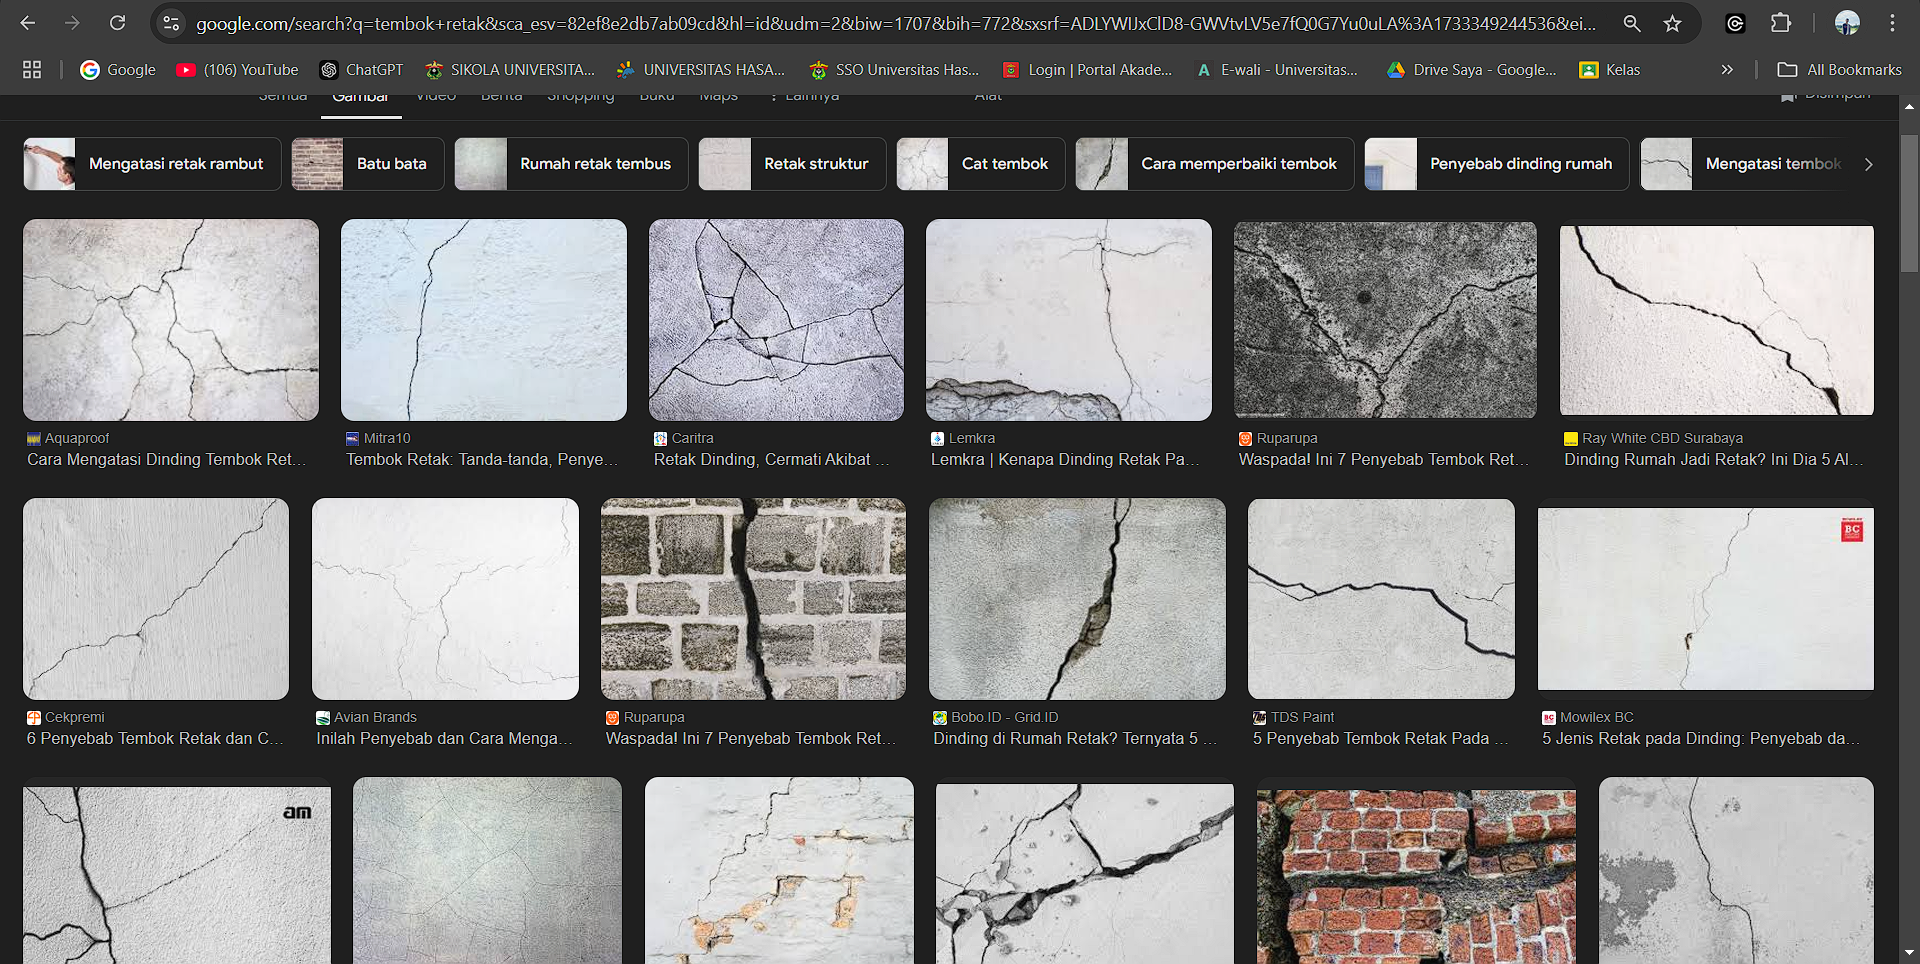
\includegraphics[width=0.6\linewidth]{Images/google.png}
        \caption*{Gambar 2. Pengambilan Gambar Di Google Images}
        \label{fig:enter-label}
    \end{figure}
    \item IStockPhoto: Gambar berlisensi dari iStockPhoto digunakan untuk memperkaya keragaman dataset.
    \begin{figure}[h]
        \centering
        \includegraphics[width=0.6\linewidth]{Images/istock.png}
        \caption*{Gambar 3. Pengambilan Gambar Di iStock}
        \label{fig:enter-label}
    \end{figure}
\end{itemize}

\subsubsection{Prapemrosesan Dataset}
\begin{itemize}
    \item Pembersihan Data: Gambar yang tidak relevan atau berkualitas rendah (misalnya, buram atau gelap) dihapus.
    \item Augmentasi Dataset: Dilakukan anotasi terhadap seluruh gambar kemudian ukurannya disesuaikan menjadi 600 x 600 piksel.
    \item Anotasi (Labeling): Gambar yang telah dikumpulkan diunggah ke platform \textit{Roboflow} untuk anotasi manual. Setiap gambar diberi label berdasarkan tiga kategori: 
    \begin{itemize}
        \item Berlubang: Kerusakan berupa lubang di permukaan jalan.
        \item Retak: Pola keretakan seperti retak memanjang, laba-laba, atau melintang.
        \item Lainnya: Kerusakan lain seperti jalan bergelombang atau gembung.
        \begin{figure}[h]
            \centering
            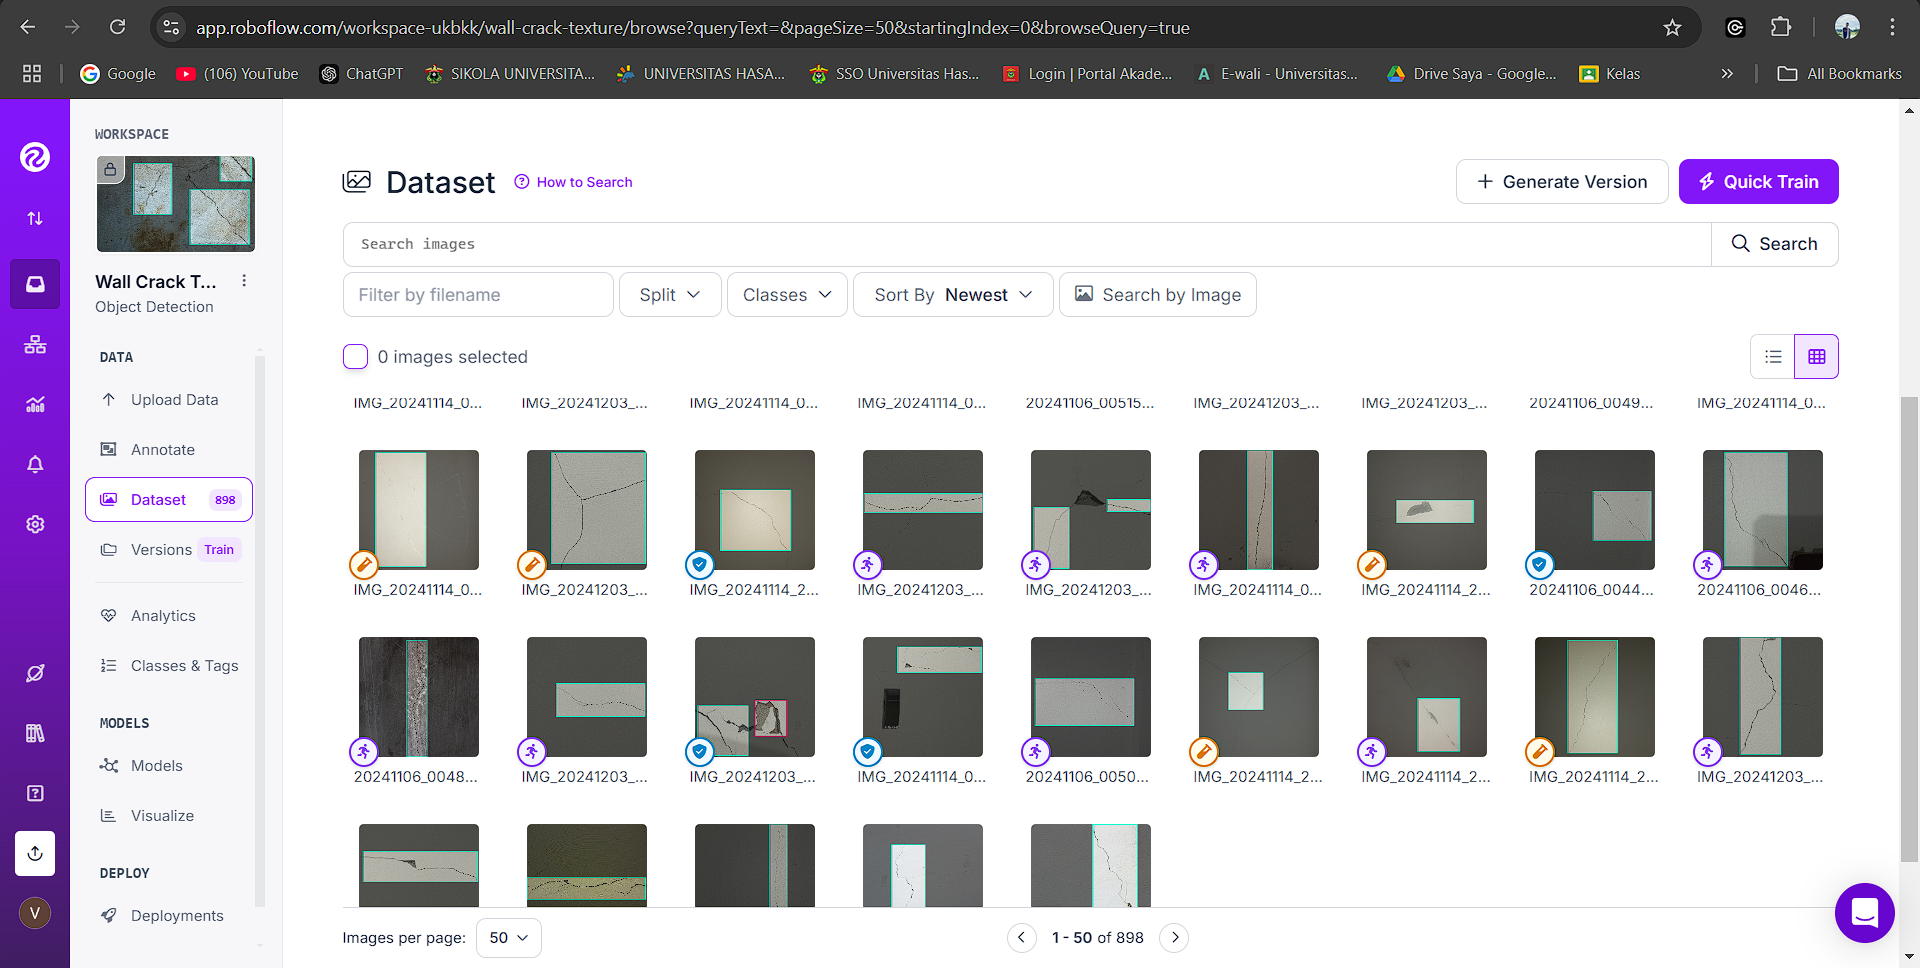
\includegraphics[width=0.8\linewidth]{Images/labeling.png}
            \caption*{Gambar 4. Anotasi di Roboflow}
            \label{fig:enter-label}
        \end{figure}
    \end{itemize}
\end{itemize}

\subsubsection{Karakteristik Dataset}
\begin{itemize}
    \item Jumlah Label:
    \begin{itemize}
        \item Berlubang: 591 label.
        \item Retak: 530 label.
        \item Lainnya: 324 label.
        \begin{figure}[h]
            \centering
            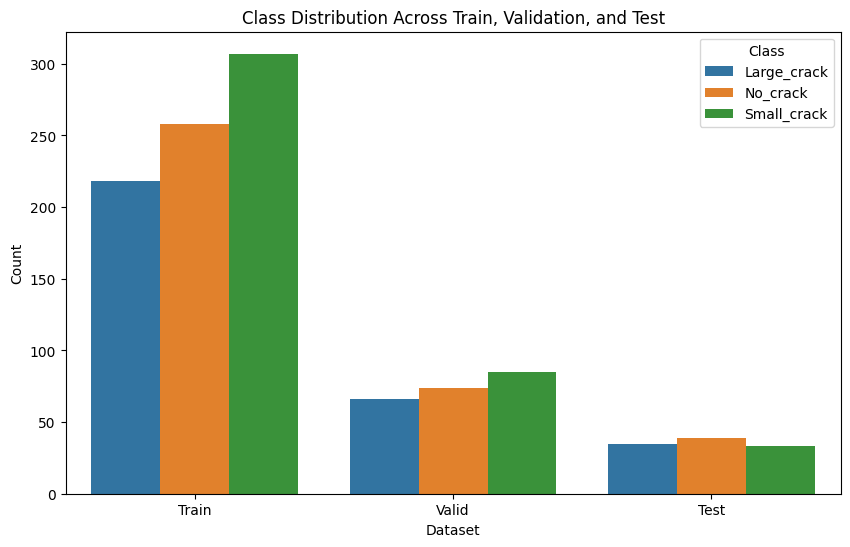
\includegraphics[width=0.9\linewidth]{Images/jumlahlabel.png}
            \caption*{Gambar 5. Distribusi Kelas Train, Validasi dan Test}
            \label{fig:enter-label}
        \end{figure}
    \end{itemize}
    \item Total Dataset: 842 gambar setelah pembersihan data.
    \item Proporsi Data Berdasarkan Label:
    \begin{itemize}
        \item Berlubang: 40\%.
        \item Retak: 40\%.
        \item Lainnya: 20\%.
    \end{itemize}
    \item Format File: Semua gambar disimpan dalam format JPG/PNG dengan anotasi dalam format YOLO (bounding box).
\end{itemize}

\subsection{Material dan Alat}

\subsubsection{Alat dan Platform Anotasi}
\begin{itemize}
    \item Roboflow: Digunakan untuk mengunggah gambar, melakukan anotasi, dan mengelola dataset. Anotasi diekspor dalam format YOLO untuk mempermudah pelatihan model.
    \item Google Colab: Untuk pelatihan model menggunakan GPU gratis.
\end{itemize}

\subsubsection{Pustaka dan Kerangka Kerja}
\begin{itemize}
    \item YOLOv5: Model deteksi objek yang digunakan untuk mendeteksi dan mengklasifikasikan kerusakan jalan.
    \item Numpy dan Pandas: Untuk manipulasi data selama analisis \textit{dataset}.
\end{itemize}

% 4. Result and Discussion
\section{RESULT AND DISCUSSION}
\subsection{Performance Metrics}

% Tabel dengan kategori "Lainnya"
\begin{table}[ht]
\centering
\begin{tabularx}{0.7\textwidth}{lCCCC}
    \toprule
    \textbf{Label} & \textbf{mAP50} & \textbf{Precision} & \textbf{Recall} & \textbf{F1 Score} \\
    \midrule
    Retak & 0.300 & 0.432 & 0.349 & 0.386 \\
    Berlubang & 0.607 & 0.586 & 0.542 & 0.563 \\
    Lainnya & 0.266 & 0.384 & 0.285 & 0.327 \\
    All & 0.391 & 0.467 & 0.392 & 0.426 \\
    \bottomrule
\end{tabularx}
\caption{Metrik Evaluasi Model Dengan Kelas "Lainnya".}
\label{tab:with_others}
\end{table}
\begin{adjustwidth}{3em}{0pt} 
Dalam hal ini penggunaan YOLOv3 tidak digunakan karena tidak berhasil setiap kali dilatih. Tabel diatas menunjukkan performa model YOLOv5 dalam mendeteksi tiga kategori kerusakan jalan: Retak, Berlubang, dan Lainnya (kerusakan yang tidak masuk dalam dua kategori utama). Metrik yang digunakan adalah:

\begin{itemize}
    \item mAP50 (mean Average Precision at IoU threshold 0.5): Mengukur rata-rata presisi untuk semua kategori pada threshold IoU 0.5. Nilai ini menunjukkan seberapa akurat prediksi model dalam menentukan lokasi kerusakan. Pada tabel, kategori Berlubang memiliki nilai mAP50 tertinggi (0.607), yang menunjukkan performa model sangat baik untuk mendeteksi Berlubang. Namun, performa untuk kategori Lainnya lebih rendah (0.266).
    
    \item Precision: Mengukur akurasi prediksi model, yaitu proporsi prediksi kerusakan yang benar dari semua prediksi kerusakan. Model memiliki presisi tertinggi untuk Berlubang (0.586), diikuti oleh Retak (0.432). Kategori Lainnya memiliki presisi terendah (0.384), menunjukkan banyak prediksi pada kategori ini yang salah.
    
    \item Recall: Mengukur kemampuan model dalam mendeteksi kerusakan yang benar, yaitu proporsi kerusakan yang benar-benar terdeteksi dari seluruh kerusakan yang ada. Recall tertinggi adalah pada Berlubang (0.542), sedangkan Lainnya memiliki nilai terendah (0.285), menunjukkan bahwa model kurang mampu mendeteksi kategori ini.
    
    \item F1-Score: Kombinasi dari Precision dan Recall, yang memberikan keseimbangan antara keduanya. F1-Score tertinggi ada pada kategori Berlubang (0.563), sedangkan kategori Lainnya kembali menunjukkan performa terendah (0.327).
    
    \item Interpretasi: Model bekerja dengan baik untuk kategori Berlubang, dengan mAP50, Precision, Recall, dan F1-Score yang cukup tinggi. Namun, untuk kategori Lainnya, performa menurun drastis, menunjukkan bahwa model kesulitan menggeneralisasi kategori ini. 
\end{itemize}
\end{adjustwidth}

% Tabel tanpa kategori "Lainnya"
\begin{table}[ht]
\centering
\begin{tabularx}{0.7\textwidth}{lCCCC}
    \toprule
    \textbf{Label} & \textbf{mAP50} & \textbf{Precision} & \textbf{Recall} & \textbf{F1 Score} \\
    \midrule
    Retak & 0.240 & 0.443 & 0.302 & 0.359 \\
    Berlubang & 0.631 & 0.601 & 0.658 & 0.628 \\
    All & 0.436 & 0.522 & 0.480 & 0.500 \\
    \bottomrule
\end{tabularx}
\caption{Metrik Evaluasi Model Tanpa Kelas "Lainnya".}
\label{tab:without_others}
\end{table}

\begin{adjustwidth}{3em}{0pt}
Tabel diatas menunjukkan performa model hanya pada dua kategori utama, yaitu Retak dan Berlubang, tanpa mempertimbangkan kategori Lainnya. Hasilnya:

\begin{itemize}
    \item mAP50: Tanpa kategori Lainnya, mAP50 untuk Berlubang meningkat menjadi 0.631 (dari 0.607), sedangkan Retak sedikit menurun menjadi 0.240 (dari 0.300). Hal ini menunjukkan bahwa kategori Lainnya memengaruhi akurasi model secara keseluruhan.
    
    \item Precision: Precision meningkat untuk kedua kategori. Retak memiliki nilai presisi 0.443, sedangkan Berlubang mencapai 0.601. Dengan menghapus kategori Lainnya, model lebih konsisten dalam menghasilkan prediksi yang benar.
    
    \item Recall: Nilai Recall juga meningkat untuk kedua kategori. Berlubang menunjukkan nilai tertinggi (0.658), yang berarti model lebih baik dalam mendeteksi kerusakan jalan berlubang.
    
    \item F1-Score: Kombinasi Precision dan Recall menunjukkan peningkatan performa pada kedua kategori, dengan nilai tertinggi untuk Berlubang (0.628). Kategori Retak memiliki F1-Score lebih rendah (0.359), tetapi tetap lebih baik dibandingkan tabel pertama.
    
    \item Interpretasi: Menghapus kategori Lainnya meningkatkan performa model pada kategori utama, Retak dan Berlubang. Model tidak lagi "terganggu" oleh kategori yang sulit dideteksi, sehingga prediksi menjadi lebih akurat dan konsisten. 
\end{itemize}
\end{adjustwidth}

\begin{figure}[h]
    \centering
    \includegraphics[width=0.6\linewidth]{Images/confusionmatrix_w.jpg}
    \caption*{Gambar 6. Confusion Matrix Dengan Kelas "Lainnya"}
    \label{fig:enter-label}
\end{figure}
\begin{adjustwidth}{3em}{0pt}
\hspace{0.5cm} Pada gambar confusion matrix diatas mencakup empat kelas yaitu berlubang, retak, background, dan lainnya. Penambahan kelas lainnya memungkinkan model untuk mengklasifikasikan sampel yang tidak termasuk ke dalam kelas utama sebagai kategori khusus, sehingga membantu menangani data yang sulit diidentifikasi. Hasilnya menunjukkan bahwa model memiliki performa cukup baik untuk kelas berlubang (68 prediksi benar) dan background (62 prediksi benar). Namun, beberapa kesalahan signifikan terjadi, misalnya banyak sampel dari kelas berlubang yang salah diklasifikasikan sebagai background (36 sampel), dan sebaliknya kelas lainnya juga mengalami misclassifications dari kelas lain seperti berlubang (7 sampel) dan background (40 sampel). Meskipun kelas lainnya mengurangi noise di kelas utama, beberapa prediksi yang salah ke kelas ini menunjukkan model belum optimal memisahkan data antar kelas.
\end{adjustwidth}

\begin{figure}[h]
    \centering
    \includegraphics[width=0.6\linewidth]{Images/confusionmatrix_wt.jpg}
    \caption*{Gambar 7. Confusion Matrix Tanpa Kelas "Lainnya"}
    \label{fig:enter-label}
\end{figure}
\begin{adjustwidth}{3em}{0pt}
\hspace{0.5cm} Sementara confusion matrix diatas hanya mencakup tiga kelas yaitu berlubang, retak, dan background, tanpa adanya kelas lainnya. Dengan pengurangan satu kelas, model dipaksa membuat keputusan yang lebih tegas antara kelas utama, tetapi ini meningkatkan risiko salah klasifikasi. Hasilnya, terlihat banyak sampel dari kelas berlubang yang salah diklasifikasikan sebagai background (52 sampel), serta kebingungan antara kelas retak dan background (40 sampel). Meskipun model mampu mengidentifikasi 82 sampel dari kelas berlubang dengan benar, jumlah false positive dan false negative lebih tinggi dibandingkan gambar pertama. Ketidakhadiran kelas lainnya menyebabkan lebih banyak noise masuk ke dalam kelas utama, terutama background, sehingga menurunkan akurasi keseluruhan model.
\end{adjustwidth}

\subsection{Visualization of Results}
\begin{adjustwidth}{3em}{0pt}
\begin{figure}[h]
    \centering
    \includegraphics[width=0.6\linewidth]{Images/result_w.jpg}
    \caption*{Gambar 8. Hasil Dengan Kelas "Lainnya"}
    \label{fig:enter-label}
\end{figure}
\hspace{0.5cm} Dalam percobaan ini, dua model yang berbeda dievaluasi untuk melihat perbandingan kinerja mereka, yaitu model yang dilatih dengan kelas tambahan ("kelas lainnya") dan model yang tidak menggunakan kelas tambahan. Model pertama, yang dilatih dengan kelas tambahan, menunjukkan hasil yang stabil dalam metrik precision dan recall. Kelas tambahan ini berfungsi untuk membantu model menangani objek-objek yang tidak termasuk dalam kelas utama, dengan mengkategorikan objek yang tidak dapat terdefinisi dalam kelas lain ke dalam kategori "lainnya". Hasilnya, model ini cenderung lebih berhati-hati dalam pengklasifikasian objek, yang berdampak pada peningkatan precision. Model ini dapat menghindari kesalahan klasifikasi objek ke dalam kelas utama yang tidak relevan, meskipun ada penurunan sedikit pada recall. Penurunan recall ini terjadi karena beberapa objek yang seharusnya diklasifikasikan ke dalam kelas utama justru masuk ke dalam kategori "kelas lainnya", yang menyebabkan model kehilangan beberapa objek yang sebenarnya relevan dengan kelas utama.

\begin{adjustwidth}{3em}{0pt}
\begin{figure}[h]
    \centering
    \includegraphics[width=0.6\linewidth]{Images/result_wt.jpg}
    \caption*{Gambar 9. Hasil Tanpa Kelas "Lainnya"}
    \label{fig:enter-label}
\end{figure}
\hspace{0.5cm} 
\end{adjustwidth}

\hspace{0.5cm} Di sisi lain, model kedua, yang dilatih tanpa kelas tambahan, menunjukkan performa yang berbeda. Karena model ini hanya fokus pada kelas utama, recall-nya lebih tinggi dibandingkan dengan model pertama. Artinya, model ini lebih efektif dalam mendeteksi seluruh objek yang ada dalam kelas utama tanpa ada objek yang hilang atau terabaikan. Namun, meskipun recall meningkat, precision model ini sedikit lebih rendah. Tanpa adanya kelas tambahan untuk menangani objek yang ambigu atau tidak terklasifikasi dengan jelas, model ini cenderung lebih sering salah dalam mengklasifikasikan objek ke dalam kelas utama. Oleh karena itu, meskipun model tanpa kelas tambahan lebih baik dalam mendeteksi objek (recall), model ini juga berisiko menghasilkan lebih banyak kesalahan klasifikasi, yang mengarah pada penurunan precision.

\hspace{0.5cm}Secara keseluruhan, model dengan kelas tambahan bekerja cukup baik dalam menjaga precision yang stabil, namun menurunkan recall karena beberapa objek diklasifikasikan ke dalam kelas "lainnya". Model tanpa kelas tambahan, meskipun memiliki recall yang lebih tinggi, mengalami penurunan precision karena kurangnya kemampuan untuk mengklasifikasikan objek yang ambigu. Perbandingan ini menunjukkan bahwa penggunaan kelas tambahan dapat meningkatkan akurasi model dalam menghindari kesalahan klasifikasi, meskipun dengan sedikit penurunan kemampuan dalam mendeteksi semua objek yang relevan.
\end{adjustwidth}

\subsection{Discussion of the Results}
\begin{adjustwidth}{3em}{0pt}
\hspace{0.5cm} Hasil eksperimen ini menunjukkan adanya perbedaan performa yang signifikan antara model yang menggunakan kelas tambahan dan model yang tidak. Ketika dikaitkan dengan penelitian terdahulu, beberapa poin penting dapat diidentifikasi, terutama terkait dengan penggunaan teknik deteksi berbasis deep learning dan tantangan generalisasi dalam mendeteksi kerusakan jalan.
\begin{itemize}
    \item Pengaruh Kelas Tambahan terhadap Precision dan Recall: Pada model pertama yang menggunakan kelas tambahan, precision lebih tinggi namun recall lebih rendah. Ini sejalan dengan temuan Zhang et al. (2016), yang menemukan bahwa kesulitan utama dalam deteksi keretakan adalah kebingungan antara kerusakan dan latar belakang akibat kontras rendah. Dalam model kami, kelas tambahan membantu menangani objek yang ambigu atau sulit diklasifikasikan, yang secara efektif meningkatkan precision karena model dapat mengklasifikasikan sampel yang tidak sesuai ke dalam kelas "lainnya." Ini mirip dengan solusi Zhang et al. yang mencoba meningkatkan precision dengan mengatasi noise. Namun, kelemahan dari pendekatan ini adalah penurunan recall, karena beberapa objek yang relevan diklasifikasikan sebagai "lainnya" alih-alih kelas target.

    \item Efek Penghapusan Kelas Tambahan pada Recall: Pada model kedua, recall yang lebih tinggi diperoleh dengan menghilangkan kelas tambahan. Ini menunjukkan bahwa model lebih berhasil dalam mendeteksi semua objek di kelas utama, tetapi dengan pengorbanan pada precision. Temuan ini menggemakan penelitian Maeda et al. (2018), yang menggunakan transfer learning dan juga mengalami masalah dalam mengurangi false positives ketika model dihadapkan pada lingkungan yang lebih kompleks. Tanpa adanya kelas tambahan, model kedua cenderung salah mengklasifikasikan objek yang ambigu sebagai kelas utama, yang menghasilkan penurunan precision, tetapi model ini lebih responsif dalam mendeteksi semua objek yang relevan (higher recall).

    \item Tantangan Deteksi Keretakan dan Noise pada Kelas Background: Hasil confusion matrix menunjukkan bahwa model tanpa kelas tambahan mengalami lebih banyak kesalahan klasifikasi, terutama dalam membedakan antara kelas berlubang dan background. Hal ini serupa dengan tantangan yang diidentifikasi oleh Zou et al. (2018) dalam model DeepCrack, di mana deteksi retakan lebih sulit karena sifatnya yang halus dan kurang jelas dibandingkan dengan lubang jalan yang lebih tegas. Dalam eksperimen ini, tanpa adanya kelas tambahan, noise lebih sering masuk ke dalam kelas background, sehingga memperburuk kesalahan klasifikasi pada model kedua, yang mengarah pada lebih banyak false positives dan false negatives.

    \item Peningkatan Recall pada Kelas Utama dengan Mengurangi Kelas Ambigu: Penelitian oleh Yang et al. (2020), yang menggunakan pendekatan piramida fitur, juga menghadapi tantangan dalam menangani variasi kondisi jalan dan aplikasi real-time. Dalam kasus ini, meskipun model kedua meningkatkan recall untuk kelas utama (berlubang), ketidakhadiran kelas tambahan menyebabkan peningkatan noise dalam klasifikasi. Ini menunjukkan bahwa meskipun recall meningkat, tantangan tetap ada dalam hal generalisasi model untuk membedakan kelas-kelas yang memiliki fitur serupa, seperti yang ditemukan dalam studi Yang et al.

    \item Keuntungan dan Keterbatasan Model Berbasis YOLO: Penelitian Bučko et al. (2022) menunjukkan bahwa model YOLOv5 sangat efektif dalam mendeteksi lubang jalan dalam kondisi yang sulit. Ini konsisten dengan hasil yang diperoleh dalam eksperimen ini, di mana YOLOv5 menunjukkan performa yang baik dalam mendeteksi kelas berlubang. Namun, seperti yang diamati dalam confusion matrix, model mengalami kesulitan dalam membedakan kerusakan yang lebih halus seperti retakan, terutama ketika kelas tambahan tidak digunakan. Meskipun YOLOv5 unggul dalam deteksi objek yang jelas seperti lubang jalan, tantangan tetap ada dalam meningkatkan akurasi deteksi kerusakan jalan yang lebih samar.

    \item Pentingnya Penggunaan Dataset yang Beragam: Cano-Ortiz et al. (2024) menekankan pentingnya dataset yang besar dan beragam untuk mengoptimalkan kinerja model deteksi kerusakan jalan. Dalam konteks penelitian ini, penggunaan kelas tambahan membantu dalam menangani sampel yang tidak cocok atau sulit diidentifikasi, yang pada gilirannya mengurangi kebingungan antara kelas utama. Hasil ini menekankan pentingnya memiliki data yang lebih representatif, terutama untuk kategori "lainnya," sehingga model dapat lebih akurat dalam menangani variasi kondisi jalan dan jenis kerusakan yang lebih kompleks. \end{itemize}

\hspace{0.5cm} Secara keseluruhan, penggunaan kelas tambahan terbukti membantu meni-ngkatkan precision dengan mengurangi kesalahan klasifikasi ke dalam kelas utama, tetapi hal ini juga menyebabkan penurunan recall karena beberapa objek yang relevan diklasifikasikan sebagai "lainnya." Di sisi lain, penghapusan kelas tambahan meningkatkan recall tetapi menyebabkan penurunan precision karena peningkatan false positives. Temuan ini konsisten dengan berbagai studi terdahulu yang menekankan tantangan deteksi kerusakan jalan, terutama dalam menangani kerusakan halus seperti retakan, dan menunjukkan bahwa penggunaan metode deteksi yang lebih canggih atau dataset yang lebih beragam diperlukan untuk mengoptimalkan kinerja model dalam berbagai kondisi jalan.

\end{adjustwidth}

% 5. Conclusion
\section{CONCLUSION}
\begin{adjustwidth}{3em}{0pt}
\subsection{Rekap Tujuan dan Pencapaian}
\hspace{0.5cm} Proyek ini bertujuan untuk menghasilkan dataset kerusakan jalan yang mencakup informasi detail tentang jalan berlubang, retak, dan jenis kerusakan lainnya, serta menggunakan teknik Deep Learning dengan model YOLOv5 untuk mendeteksi kerusakan jalan secara otomatis. Tujuan ini berhasil dicapai melalui:
\begin{itemize}
    \item Pengembangan dataset yang kaya akan informasi terkait jenis kerusakan jalan, termasuk lubang jalan dan retakan, menggunakan gambar dari berbagai kondisi lingkungan.
    \item Implementasi model YOLOv5 yang dapat mendeteksi kerusakan jalan dengan tingkat akurasi yang cukup.
\end{itemize}

\subsection{Wawasan Utama dari Hasil}
\begin{itemize}
    \item Efektivitas Model Deep Learning: Model YOLOv5 menunjukkan performa yang cukup, terutama dalam kondisi pencahayaan rendah dan visibilitas yang menantang.
    \item Kondisi Lingkungan yang Berpengaruh: Faktor seperti hujan, malam hari, dan genangan air memengaruhi akurasi deteksi, menunjukkan pentingnya augmentasi data dan pengembangan algoritma yang lebih tangguh untuk kondisi tersebut.
    \item Potensi Integrasi dengan Teknologi Real-Time: Penggunaan model deteksi ini bersama sensor kendaraan memiliki potensi untuk meningkatkan keselamatan berkendara secara signifikan dengan memberikan peringatan dini kepada pengemudi.
    \item Dampak pada Perkembangan Kendaraan Otonom: Dataset dan model yang dihasilkan memberikan kontribusi penting dalam mendukung teknologi kenda-raan otonom, terutama dalam kemampuan navigasi di jalan yang tidak rata.
\end{itemize}

\subsection{Pekerjaan dan Rekomendasi di Masa Depan}
\begin{itemize}
    \item Pengembangan Dataset Lebih Lanjut: Perluasan dataset dengan menambahkan lebih banyak gambar dari berbagai kondisi lingkungan ekstrem, seperti kabut, atau kondisi jalan berlumpur, untuk meningkatkan robusta model.
    \item Peningkatan Model Deep Learning: Penelitian lebih lanjut dapat difokuskan pada pengembangan atau fine-tuning model yang lebih canggih, seperti YOLO-v7 atau Transformer-based models, untuk meningkatkan akurasi deteksi pada kondisi pencahayaan rendah.
    \item Integrasi dengan Teknologi Sensor Kendaraan: Melakukan uji coba lapangan untuk mengintegrasikan model ini dengan teknologi sensor kendaraan dan sistem GPS untuk memberikan deteksi kerusakan jalan secara real-time.
    \item Sistem Deteksi Terdistribusi: Mengembangkan sistem berbasis cloud yang memungkinkan berbagi informasi kerusakan jalan secara otomatis antara pengguna jalan, pemerintah, dan penyedia layanan kendaraan.
    \item Kolaborasi dengan Pemangku Kepentingan: Menjalin kerja sama dengan instansi pemerintah, produsen kendaraan otonom, dan penyedia layanan transportasi untuk mengadopsi teknologi ini dalam sistem pengelolaan jalan yang lebih luas.
\end{itemize}
\hspace{0.5cm} Proyek ini menjadi landasan penting dalam memanfaatkan teknologi visi komputer dan deep learning untuk menciptakan solusi berkelanjutan di bidang infrastruktur jalan, yang pada akhirnya dapat meningkatkan kualitas hidup masyarakat dan keselamatan berkendara secara keseluruhan.

\end{adjustwidth}
\newpage
\begin{thebibliography}{99}
\begin{enumerate}
    \item Bučko, B.; Lieskovská, E.; Zábovská, K.; Zábovský, M. Computer Vision Based Pothole Detection under Challenging Conditions. \textit{Sensors} \textbf{2022}, \textit{22}, 8878.  
    Available online: \url{https://doi.org/10.3390/s22228878} (accessed on 17 November 2022).

    \item Cano-Ortiz, S.; Lloret Iglesias, L.; Martinez Ruiz del Árbol, P.; Lastra-González, P.; Castro-Fresno, D. An End-to-End Computer Vision System Based on Deep Learning for Pavement Distress Detection and Quantification. \textit{Construction and Building Materials} \textbf{2024}, \textit{416}, 135036.  
    Available online: \url{https://www.elsevier.com/locate/conbuildmat} (accessed on 2 February 2024).
    
    \item Gopalakrishnan, K.; Khaitan, S.K.; Choudhary, A.; Agrawal, A. Deep Convolutional Neural Networks with Transfer Learning for Computer Vision-Based Data-Driven Pavement Distress Detection. \textit{Construction and Building Materials} \textbf{2017}, \textit{157}, 322–330.  
    Available online: \url{https://www.sciencedirect.com/science/article/abs/pii/S0950061817319335} (accessed on 30 December 2017).
    
    \item Maeda, H.; Sekimoto, Y.; Seto, T.; Kashiyama, T.; Omata, H. Road Damage Detection and Classification Using Deep Neural Networks with Smartphone Images. \textit{Journal of Computer-Aided Civil Infrastructure Engineering} \textbf{2018}.  
    Available online: \url{https://onlinelibrary.wiley.com/doi/full/10.1111/mice.12387} (accessed on 30 June 2018).
    
    \item Yang, F.; Zhang, L.; Yu, S.; Prokhorov, D.; Mei, X.; Ling, H. Feature Pyramid and Hierarchical Boosting Network for Pavement Crack Detection. \textit{IEEE Transactions on Image Processing} \textbf{2020}.  
    Available online: \url{https://ieeexplore.ieee.org/document/8694955} (accessed on 2020).
    
    \item Zhang, L.; Yang, F.; Zhang, Y.D.; Zhu, Y.J. Road Crack Detection Using Deep Convolutional Neural Network. \textit{IEEE Transactions on Intelligent Transportation Systems} \textbf{2016}.  
    Available online: \url{https://ieeexplore.ieee.org/document/7533052} (accessed on 2016).
    
    \item Zhang, A.; Wang, K.C.P.; Li, B.; Yang, E.; Dai, X.; Peng, Y.; Fei, Y.; Liu, Y.; Li, J.Q.; Chen, C. Automated Pixel-Level Pavement Crack Detection on 3D Asphalt Surfaces Using a Deep-Learning Network. \textit{Journal of Computer-Aided Civil Infrastructure Engineering} \textbf{2017}.  
    Available online: \url{https://onlinelibrary.wiley.com/doi/full/10.1111/mice.12297} (accessed on 2017).
    
    \item Zou, Q.; Zhang, Z.; Li, Q.; Qi, X.; Wang, Q.; Wang, S. DeepCrack: Learning Hierarchical Convolutional Features for Crack Detection. \textit{IEEE Transactions on Image Processing} \textbf{2019}.  
    Available online: \url{https://ieeexplore.ieee.org/document/8517148} (accessed on 2019).
    
\end{enumerate}
\end{thebibliography}
\end{document}